\documentclass[11pt]{article}

\usepackage[margin = 0.75in]{geometry} 

\setlength{\parindent}{0cm}


\usepackage{tikz}
\usetikzlibrary{calc}
\usepackage{ifthen}

\begin{document}

\begin{center}
  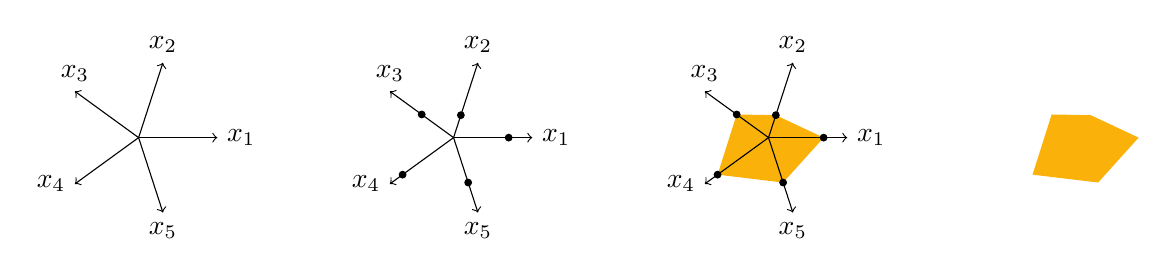
\begin{tikzpicture}
  [dot/.style={shape = circle, fill=black,inner sep = 1pt}]

  \newcommand{\radius}{1}
  \newcommand{\dist}{4}

    \begin{scope}
      \coordinate (x1) at (0:\radius);
      \coordinate (x2) at (72:\radius);
      \coordinate (x3) at (144:\radius);
      \coordinate (x4) at (216:\radius);
      \coordinate (x5) at (288:\radius);

      \draw[->] (0,0) -- (x1) node [right] {$x_1$};
      \draw[->] (0,0) -- (x2) node [ above] {$x_2$};
      \draw[->] (0,0) -- (x3) node [ above] {$x_3$};
      \draw[->] (0,0) -- (x4) node [ left] {$x_4$};
      \draw[->] (0,0) -- (x5) node [ below] {$x_5$};
    \end{scope}

    \begin{scope}[shift={(\dist,0)}]


      \coordinate (x1) at (0:\radius);
      \coordinate (x2) at (72:\radius);
      \coordinate (x3) at (144:\radius);
      \coordinate (x4) at (216:\radius);
      \coordinate (x5) at (288:\radius);

      \draw[->] (0,0) -- (x1) node [right] {$x_1$};
      \draw[->] (0,0) -- (x2) node [ above] {$x_2$};
      \draw[->] (0,0) -- (x3) node [ above] {$x_3$};
      \draw[->] (0,0) -- (x4) node [ left] {$x_4$};
      \draw[->] (0,0) -- (x5) node [ below] {$x_5$};


      \node at ($(0,0)!0.7!(x1)$) [dot] {};
      \node at ($(0,0)!0.3!(x2)$) [dot] {};
      \node at ($(0,0)!0.5!(x3)$) [dot] {};
      \node at ($(0,0)!0.8!(x4)$) [dot] {};
      \node at ($(0,0)!0.6!(x5)$) [dot] {};

    \end{scope}

    \begin{scope}[shift={(2*\dist,0)}]
      \coordinate (x1) at (0:\radius);
      \coordinate (x2) at (72:\radius);
      \coordinate (x3) at (144:\radius);
      \coordinate (x4) at (216:\radius);
      \coordinate (x5) at (288:\radius);

      \fill [fill = yellow!40!orange] ($(0,0)!0.7!(x1)$) -- ($(0,0)!0.3!(x2)$) -- ($(0,0)!0.5!(x3)$) -- ($(0,0)!0.8!(x4)$) -- ($(0,0)!0.6!(x5)$) -- cycle;
      
      
      \draw[->] (0,0) -- (x1) node [right] {$x_1$};
      \draw[->] (0,0) -- (x2) node [ above] {$x_2$};
      \draw[->] (0,0) -- (x3) node [ above] {$x_3$};
      \draw[->] (0,0) -- (x4) node [ left] {$x_4$};
      \draw[->] (0,0) -- (x5) node [ below] {$x_5$};

      \node at ($(0,0)!0.7!(x1)$) [dot] {};
      \node at ($(0,0)!0.3!(x2)$) [dot] {};
      \node at ($(0,0)!0.5!(x3)$) [dot] {};
      \node at ($(0,0)!0.8!(x4)$) [dot] {};
      \node at ($(0,0)!0.6!(x5)$) [dot] {};


    \end{scope}


    \begin{scope}[shift = {(3*\dist,0)}]
      \coordinate (x1) at (0:\radius);
      \coordinate (x2) at (72:\radius);
      \coordinate (x3) at (144:\radius);
      \coordinate (x4) at (216:\radius);
      \coordinate (x5) at (288:\radius);

      \fill [fill = yellow!40!orange] ($(0,0)!0.7!(x1)$) -- ($(0,0)!0.3!(x2)$) -- ($(0,0)!0.5!(x3)$) -- ($(0,0)!0.8!(x4)$) -- ($(0,0)!0.6!(x5)$) -- cycle;

    \end{scope}

    
  \end{tikzpicture}
\end{center}


%%%%%%%%%%%%%%%%%%%%%%%%%%%%%%%%%%%%%%%%%%%

%% Graph Data Viz relationship

\begin{center}
  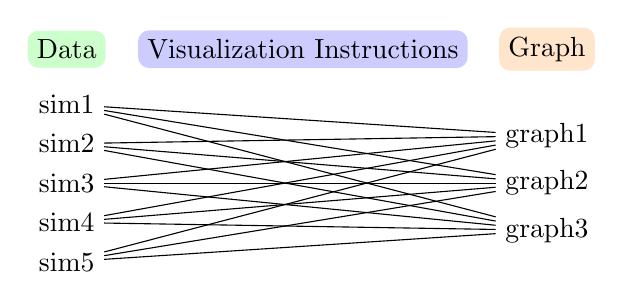
\begin{tikzpicture}
    \node at (0,0) [fill=green!20, rounded corners] {Data};
    \node at (3,0) [fill=blue!20, rounded corners] {Visualization Instructions};
    \node at (6.1,0) [fill=orange!20, rounded corners] {Graph};

    \node (s1) at (0,-0.7) {sim1};
    \node (s2) at (0,-1.2) {sim2};
    \node (s3) at (0,-1.7) {sim3};
    \node (s4) at (0,-2.2) {sim4};
    \node (s5) at (0,-2.7) {sim5};

    \node (g1) at (6.1,-1.1) {graph1};
    \node (g2) at (6.1,-1.7) {graph2};
    \node (g3) at (6.1,-2.3) {graph3};
    
    \foreach \graph in {g1,g2,g3} {
      \foreach \data in {s1,s2,s3,s4,s5} {
        \draw  (\graph) -- (\data);
      }
    }   
  \end{tikzpicture}
\end{center}


\begin{center}
  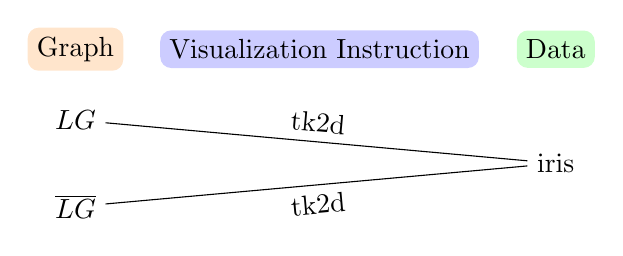
\begin{tikzpicture}
    \node at (6.1,0) [fill=green!20, rounded corners] {Data};
    \node at (3.1,0) [fill=blue!20, rounded corners] {Visualization Instruction};
    \node at (0,0) [fill=orange!20, rounded corners] {Graph};

    \node (g1) at (0,-0.9) {$LG$};
    \node (g2) at (0,-2) {$\overline{LG}$};
    
    \node (s1) at (6.1,-1.45) {iris};

    \draw (g1) -- (s1) node [above,midway,sloped] {tk2d};
    \draw (g2) -- (s1) node [below,midway,sloped] {tk2d};
  \end{tikzpicture}
\end{center}  

\begin{center}
\begin{tabular}{|p{4cm}|p{4cm}|p{4cm}|}
  \hline 
  \textbf{color} & \textbf{interaction} & \textbf{display}\\
  \hline
   background       &    bulletRadius          &   NSteps            \\
   bullet           &    nodeRadius            &   animationSpeed    \\
   bulletActive     &    lineWidth             &   dragSelectRadius  \\
   nodes            &    highlightedLineWidth  &   labelDistRadius   \\
   nodesActive      &                          &                     \\
   adjNodes         &                          &                     \\
   adjNodesActive   &                          &                     \\
   notVisitedEdge   &                          &                     \\
   visitedEdge      &                          &                     \\
   edgeActive       &                          &                     \\
   labels           &                          &                     \\
   labelsActive     &                          &                     \\
   adjLabels        &                          &                     \\
   adjLabelsActive  &                          &                     \\
   path             &                          &                     \\
   \hline
\end{tabular}
\end{center}


	
        
        
         
        
   
   
   
    
        
        


%%%%%%%%%%%%%%%%%%%%%%%%%%%%%%%%%%%%%%%%%%%



\newcommand{\ngwindow}{
\fill [fill=gray!40] (0,0) rectangle (\ww,-0.2);
\fill [fill=brown!10] (0,-0.2) rectangle (\ww,-0.4);
\draw (0,0) rectangle (\ww,-\wh);
\draw (0,-0.2) -- (\ww,-0.2);
\draw (0,-0.4) -- (\ww,-0.4);
}

\newcommand{\nggraph}[9]{
  \begin{scope}[shift= {(2,-3.6/2-0.4)}]
    \node at ( 1, 0)  [#1, label=right:{\scriptsize A:B}] (AB) {};
    \node at ( 0, -1) [#2, label=below:{\scriptsize A:D}] (AD) {};
    \node at (-1, 0)  [#3, label=left:{\scriptsize B:C}] (BC) {};
    \node at ( 0, 1)  [#4, label=above:{\scriptsize C:D}] (CD) {};
    \draw[#5] (AB) -- (AD);
    \draw[#6] (AB) -- (BC);
    \draw[#7] (AB) -- (CD);
    \draw[#8] (AD) -- (BC);
    \draw[#9] (AD) -- (CD);
  \end{scope}
}

\newcommand{\ww}{4}
\newcommand{\wh}{4}

\newcommand{\mouse}[4]{
  \begin{scope}[shift={#1}]
    \filldraw[fill=white, draw = black, line width=1pt] (0,0) -- (-90:0.45) -- (-75:0.35) -- (-70:0.5) -- (-57:0.5) -- (-55:0.35) -- (-40:0.45) -- cycle; 
    \ifthenelse{\equal{#2}{}}{}{\node at #3 [#4, fill=red!30, line width = 1pt, draw = red!50!black, rounded corners] {#2};}
  \end{scope}
}



\begin{center}
  \begin{tikzpicture}
 [a/.style={circle, draw=black!50, fill=purple!80, minimum size=3mm},
  na/.style={circle, draw=black!50, fill=violet!100, minimum size=3mm},
  bullet/.style={circle, draw=black, fill=yellow!80,thick, minimum size=5mm},
  nc/.style={draw=black!30,line width=1.5pt},
  co/.style={draw=black!30,line width=4pt}]
    
    \begin{scope}
      \ngwindow
      \nggraph{a}{a}{a}{a}{co}{co}{co}{nc}{nc}
      \node at (AB) [bullet] {};
      \mouse{(AB)}{Left Click and Drag}{(-120:1)}{right}
      \node at (0,-0.7) [right] {0};
    \end{scope}

    \begin{scope}[shift = {(1.5*\ww,0)}]
      \ngwindow
      \nggraph{a}{na}{na}{a}{nc}{nc}{co}{nc}{nc}
      \node at ($(AB)!0.4!(CD)$) [bullet] {};
      \mouse{($(AB)!0.4!(CD)$)}{}{(-60:0.8)}{right}
      \node at (0,-0.7) [right] {40};
    \end{scope}

    \begin{scope}[shift = {(3*\ww,0)}]
      \ngwindow
      \nggraph{a}{a}{na}{a}{nc}{nc}{co}{nc}{co}
      \draw [co, draw=gray!80!black](AB) -- (CD);
      \node at (CD) [bullet] {};
      \mouse{(CD)}{}{(-60:0.8)}{right}
      \node at (0,-0.7) [right] {0};
    \end{scope}

    
  \end{tikzpicture}
\end{center}



%%%%%%%%%%%%%%%%%%%%%%%%%%%%%%%%%%%%%%%%%%%%%%%%%%%%%%%%%%%
%% drag
\begin{center}
  \begin{tikzpicture}
 [a/.style={circle, draw=black!50, fill=purple!80, minimum size=3mm},
  na/.style={circle, draw=black!50, fill=violet!100, minimum size=3mm},
  bullet/.style={circle, draw=black, fill=yellow!80,thick, minimum size=5mm},
  nc/.style={draw=black!30,line width=1.5pt},
  co/.style={draw=black!30,line width=4pt}]



    
    \begin{scope}[shift = {(3*\ww,0)}]
      \ngwindow
      \begin{scope}[shift= {(2,-3.6/2-0.4)}]


      \node at ( 1, 0)  [a, label=right:{\scriptsize A:B}] (AB) {};
      \node at ( 0, -1) [a, label=below:{\scriptsize A:D}] (AD) {};
      \node at (-1, 0)  [a, label=left:{\scriptsize B:C}] (BC) {};
      \node at ( -.5, 1)  [a] (CD) {};
      \draw[co] (AB) -- (AD);
      \draw[co] (AB) -- (BC);
      \draw[co] (AB) -- (CD);
      \draw[nc] (AD) -- (BC);
      \draw[nc] (AD) -- (CD);
      
      \node [circle, fill = blue!20, inner sep=10pt] at (CD) {};      
      \node at (CD)  [a] {};
      
      \node at (-0.8,.7) (CD1) {{\scriptsize C:D}};

    \end{scope}
      \node at (AB) [bullet] {};
      \mouse{(CD1)}{drag}{(160:0.5)}{left}
      \node at (0,-0.7) [right] {40};
    \end{scope}

    \begin{scope}[shift = {(1.5*\ww,0)}]
      \ngwindow
      \begin{scope}[shift= {(2,-3.6/2-0.4)}]
      \node at ( 1, 0)  [a, label=right:{\scriptsize A:B}] (AB) {};
      \node at ( 0, -1) [a, label=below:{\scriptsize A:D}] (AD) {};
      \node at (-1, 0)  [a, label=left:{\scriptsize B:C}] (BC) {};
      \node at ( -.5, 1)  [a, label=above:{\scriptsize C:D}] (CD) {};
      \draw[co] (AB) -- (AD);
      \draw[co] (AB) -- (BC);
      \draw[co] (AB) -- (CD);
      \draw[nc] (AD) -- (BC);
      \draw[nc] (AD) -- (CD);
    \end{scope}
      \node at (AB) [bullet] {};
      \mouse{(CD)}{drag}{(30:0.5)}{right}
      \node at (0,-0.7) [right] {0};
    \end{scope}


    \begin{scope}
      \ngwindow
      \nggraph{a}{a}{a}{a}{co}{co}{co}{nc}{nc}
      \node at (AB) [bullet] {};
      \node at (0,-0.7) [right] {0};
      \mouse{(CD)}{Ctrl Key \& Left Mouse Button}{(160:2.5)}{right}
    \end{scope}





    
  \end{tikzpicture}
\end{center}


%%%%%%%%%%%%%%%%%%%%%%%%%%%%%%%%%%%%%%%%%%%%%%%%%%%%%

\begin{center}
  \begin{tikzpicture}
 [a/.style={circle, draw=black!50, fill=purple!80, minimum size=3mm},
 p/.style={circle, draw=black!50, fill=black, minimum size=3mm},
  na/.style={circle, draw=black!50, fill=violet!100, minimum size=3mm},
  bullet/.style={circle, draw=black, fill=yellow!80,thick, minimum size=5mm},
  pbullet/.style={circle, draw=black, fill=black,thick, minimum size=5mm},
 nc/.style={draw=black!30,line width=1.5pt},
  co/.style={draw=black!30,line width=4pt}]
    

  \begin{scope}
    \ngwindow
    \nggraph{a}{a}{a}{a}{co}{co}{co}{nc}{nc}
    \node at (AB) [bullet] {};
    \node at (0,-0.7) [right] {0};
    \mouse{(CD)}{Shift \& Click}{(160:0.2)}{left}
  \end{scope}
  
  
  \begin{scope}[shift = {(1.1*\ww,0)}]
    \ngwindow
    \nggraph{a}{a}{na}{p}{nc}{nc}{co}{nc}{co}
    \draw [co, draw=black](AB) -- (CD);
    \node at (AB) [pbullet] {};
    \mouse{(AD)}{Shift \& Click}{(160:1.9)}{right}
    \node at (0,-0.7) [right] {0};
  \end{scope}

  \begin{scope}[shift = {(2.2*\ww,0)}]
    \ngwindow
    \nggraph{a}{p}{a}{p}{co}{nc}{nc}{co}{co}
    \draw [co, draw=black](CD) -- (AD);
    \mouse{(BC)}{Shift \& Double Click}{(130:0.6)}{right}
    \node at (AB) [bullet] {};
    \node at (0,-0.7) [right] {0};
  \end{scope}
  
  \begin{scope}[shift = {(3.3*\ww,0)}]
    \ngwindow
      \nggraph{a}{na}{na}{a}{nc}{nc}{co}{nc}{nc}
      
      \foreach \perc in {0.2,0.4,0.6,0.8,1} {
        \node at ($(AB)!\perc!(CD)$) [bullet] {};
      }
      \foreach \perc in {0.2,0.4,0.6,0.8,1} {
        \node at ($(CD)!\perc!(AD)$) [bullet] {};
      }
      \foreach \perc in {0.2,0.4,0.6,0.8,1} {
        \node at ($(AD)!\perc!(BC)$) [bullet] {};
      }
    \end{scope}
  \end{tikzpicture}
\end{center}


%%%%%%%%%%%%%%%%%%%%%%%%%%%%%%%%%%%%%%


\renewcommand{\ww}{9}
\renewcommand{\wh}{6}


\newcommand{\datap}{-0.8/0.5/2/violet,-0.7/0.6/2/violet,-0.56/0.36/2/violet,-0.4/0.7/2/violet,-.3/0.5/2/violet,0.2/0.3/2/red,0.3/0.5/2/red,0.5/0.7/2/red,0.43/0.34/2/red,0.54/0.55/2/red,0.6/0.12/2/red,0.33/0.16/2/red,0.49/-0.1/2/red,0.23/-.21/2/red, 0.61/-0.32/2/red,-0.5/-0.52/2/green,-0.4/-.83/2/green,-0.4/-0.35/2/green,-.58/-0.73/2/green,-0.72/-0.46/2/green,-0.23/-.69/2/green}



\begin{center}
  \begin{tikzpicture}
 
    \begin{scope}[shift = {(0,-0.4)}]
      \fill [fill = gray!20] (\ww*2/3,0) rectangle (\ww,-\wh+0.4);
      % \fill [fill = black!70] (0,0) rectangle (\ww*2/3,-\wh+0.4);

     \begin{scope}[shift = {(\ww*2/3,0)}]
        \node at (0,-0.25) [right] {Zoom: 1};
        \fill [fill=gray!40] (0.1,-0.5) rectangle (\ww/3-0.1,-2);
        
        
        \pgfmathparse{1.5/2}\let\zboxh\pgfmathresult
        \pgfmathparse{\ww/3/(\wh-0.4)*\zboxh*2}\let\zboxw\pgfmathresult
             
       
        \begin{scope}[shift = {(\ww/6,-1.25)}]
          \node at (0,0) [circle,fill=blue,inner sep=1pt] {};
          \fill [fill = white] (-\zboxw,-\zboxh) rectangle (\zboxw,\zboxh); 
          \foreach \x/\y/\size/\col in \datap {
            \node at (\x*\zboxw,\y*\zboxh) [circle, fill=\col, inner sep =1pt] {};
          }
        \end{scope}
        

        \node at (0,-2.25) [right] {Plot Type:};
        \draw (0.3,-2.6) -- (1,-2.6);
        \draw (0.3,-2.8) -- (1,-2.8);
        \node at (0,-3.2) [right] {Brush:};
        \node at (1.5,-3.2) [rectangle,fill=white,draw=black] {};
        \node at (1.7,-3.2) [right] {col:};
        \node at (2.65,-3.2) [rectangle, fill=magenta] {};            

        \node at (0,-3.75) [right] {none  all  invert};
        

        \begin{scope}[shift={(0,-4.3)}]
          \node at (0,0) [right] {col:};
          
          \foreach \x/\col in {0.25/violet,0.6/pink!40!magenta,0.95/red,1.3/blue,1.65/green,2/orange,2.35/yellow} {
            \node at (\x,-0.35) [rectangle, fill=\col] {};            
          }
          \node at (1.5,0) [right] {bg:};
          \node at (2.35,0) [rectangle, fill=white] {};            

          \node at (0,-0.7) [right] {abs:-+ rel:-+};
        \end{scope}
        

      \end{scope}
   \end{scope}


   \pgfmathparse{\ww/3.0}\let\dw\pgfmathresult
   \pgfmathparse{(\wh-0.4)/2}\let\dh\pgfmathresult

   %% Points
   \begin{scope}[shift = {(\ww/3,-.2-\wh/2)}]
        \foreach \x/\y/\size/\col in \datap {
          \node at (\x*\dw,\y*\dh) [circle, fill=\col, inner sep =\size pt] {};
        }
   \end{scope}

   
   \ngwindow
 \end{tikzpicture}
\end{center}



\end{document}
